

The TPC front-end (FE) electronics  operate at cryogenic temperatures. 
The system provides amplification, shaping,  digitization, buffering and
multiplexing of the signals. The FE electronics consist of three boards stacked on top of one another:  the Analog Mother Board, the FPGA Mezzanine Board, and the SERDES Mezzanine Board.  Figure \ref{fig:coldelec} shows a schematic of the cold FE electronics. 

\begin{figure}[tb]
  \centering
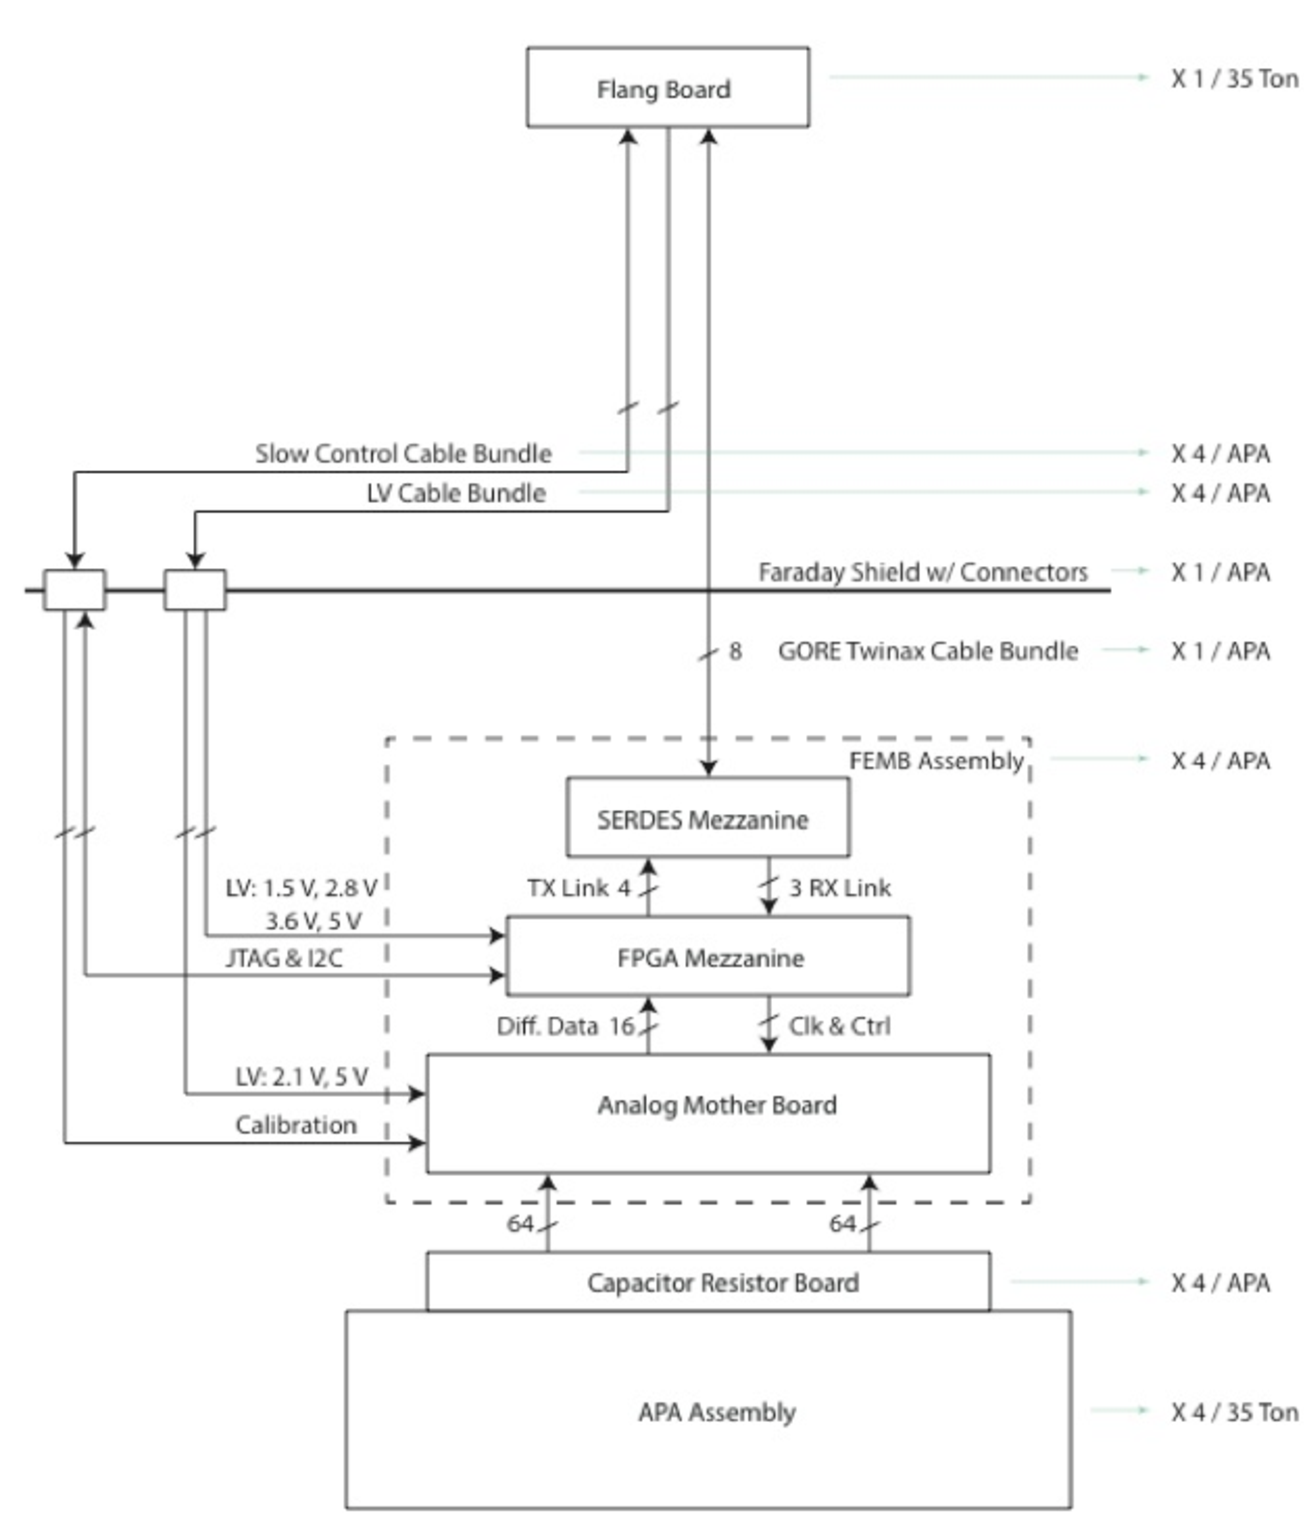
\includegraphics[scale=0.4]{figures/fe-electronics-block-diagram.pdf}
\label{fig:coldelec}
  \caption{Schematic for the TPC cold FE electronics. ***MG*** Not sure if this is high enough quality.  ***Ask Chen for source and fix numbers.  }
\end{figure}

The Analog Mother Board contains the front-end ASIC chips which perform the analog readout of the TPC wires.  The FE ASIC chip is implemented as a
mixed-signal ASIC providing amplification, shaping, digitization,
buffering, a 16:2 multiplexing stage, a driver and voltage regulators.  The analog-to-digital converter on the ASIC samples each TPC wire at 2 MHz.  Eight such chips 
are mounted on a single readout board, instrumenting 128 adjacent wires in one plane. 

The two (multiplexed) signals from each FE ASIC are fed into the FPGA Mezzanine Board.  The cold FPGA aggregates the TPC data and also supplies the control and clock to the FE ASICs.   The FPGA on the mezzanine board receives the data and packages the 128 channels together, one 2 MHz clock tick at a time.  This is then sent to the SERDES board for serialization and sent to the cryostat flange board over high-speed (1 Gbps) serial links and finally to the DAQ system.  

Besides the high-speed signal cable, which is a twin-axial cable bundle manufactured by GORE, there are cable bundles for low-voltage power, wire-bias voltages, and various slow controls and monitoring. Redundant cables will be provided for many of these functions. The  cable bundles will be connected through a feedthrough on the roof of the cryostat. 


\begin{tabular}{l|c}
\hline
 parameter & value \\
  \hline
 ADC Sampling Rate & 2 MHz\\
More stuff   & \\
 Cluster-on-Boards (COB) & 3\\
Data-Processing-Modules (DPM) & 12 \\
ATCA Shelves  & 1 (6-slot)\\
TPC Readout Compute Nodes & 3 \\
\hline
\end{tabular}



The primary interface between the TPC front-end electronics (FE) and the DAQ subsystem consists of an ATCA-based system of RCEs (Reconfigurable Cluster Elements).  The RCE system receives the serialized raw data for the FE, performs zero-suppression on it, and packetizes and transmits the resulting sparsified data to a back-end data farm for event building and further processing.  Additionally, the RCE system transmits timing and control signals to the FE as well as forwarding configuration data to them at start-up.     

The RCE system consists the following components:  a commercial ATCA shelf (2-, 6-, or 14-slot), a Cluster-On-Board (COB) which is the "front board" in ATCA terms, and a Rear-Transition-Module (RTM) which is the "rear board". A schematic of the system is shown in Figure \ref{fig:rceblock}.  The COB is a custom board, developed by SLAC, which holds the processing power of the system.  The COB (see Figure \ref{cob}) consists of 5 bays for holding daughter boards, an onboard 10-GbE switch, and both 10- and 1-Gb ethernet connections for communications with the back-end system.  Four of the daughter-board bays are for Data Processing Modules (DPM), each of which can hold up to two RCEs.  The RCE is the core procession unit of the system; it is made up of a modern SoC (currently, the Xilinx Zynq-7045) with multiple high-speed I/O ports (up to 10-Gbps each) and external DRAM and flash memory controllers.  The other bay on the COB contains the Data Transmission Module (DTM) which is responsible  for distributing timing and trigger information to and between the DPMs.  

While the COB hardware is application agnostic,  the RTM is application specific. The RTM provides the mechanical interface between the front-end (or, in our case, the flange electronics) and the back-end, as well as other external sources such as the timing or trigger systems.  In this case we will use fiber optic connections between the flange and the TPC DAQ using 8 12-channel (full duplex) CXP connectors on the RTM. 

With the assumption that each cold FE board multiplexes it's 128 wire channels to 4 outputs at 1-Gbps each, the non-zero suppressed data for 1 APA can be fed into a single COB (containing 8 RCEs).  Each RCE would receive data from 2 FE boards, perform zero-suppression, and send the result to the back-end.  

MG***data rates?  

\begin{figure}[tb]
  \centering
%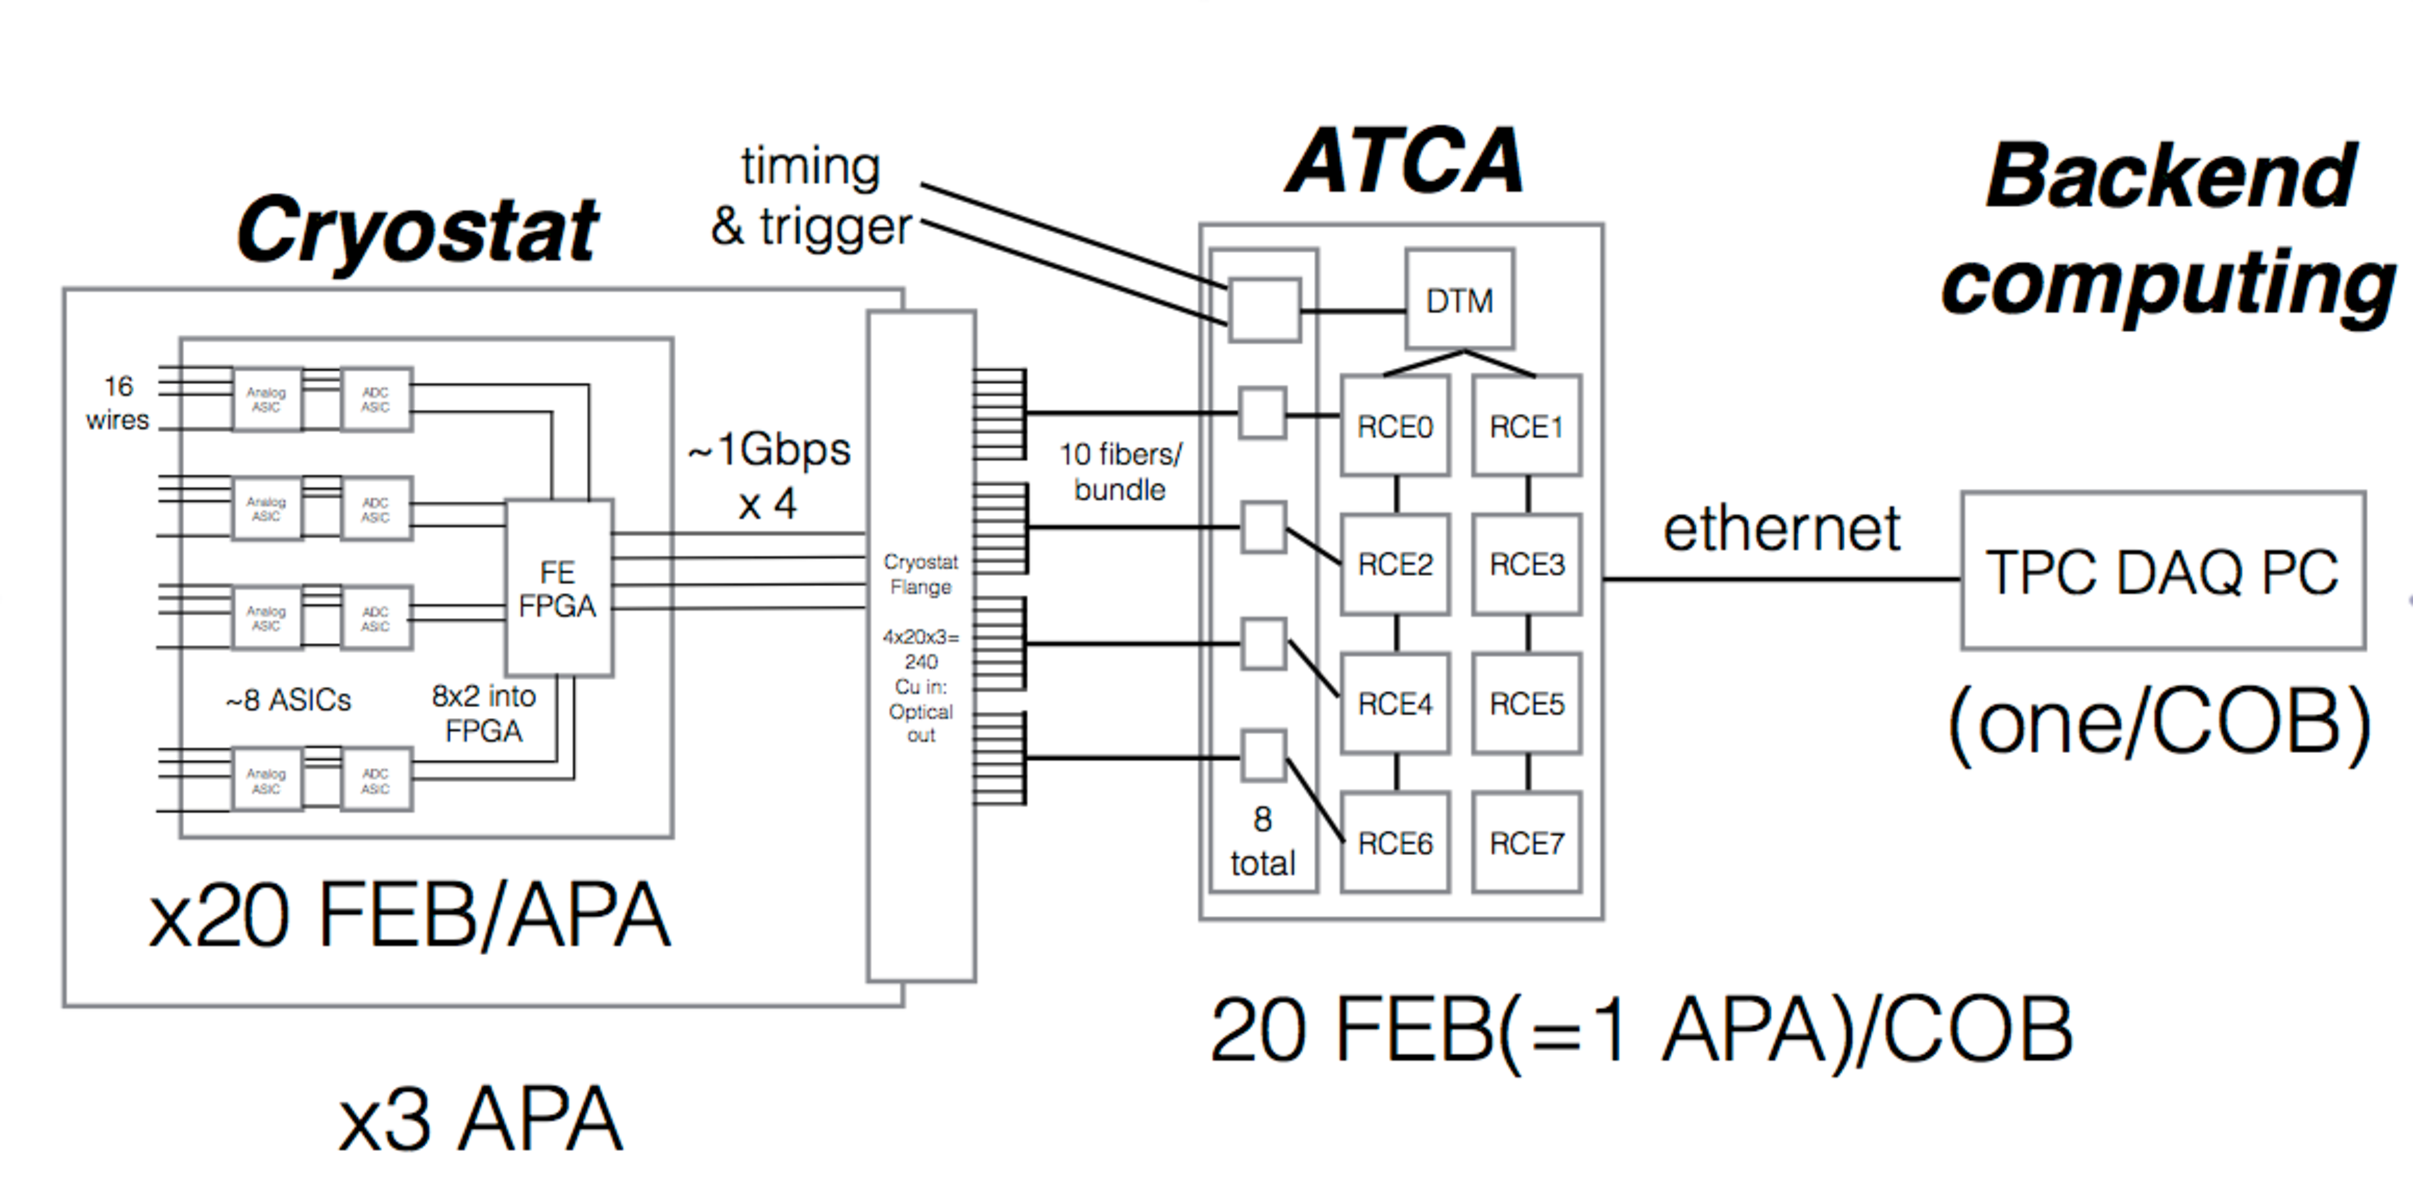
\includegraphics[scale=0.4]{figures/cern-tpc-daq-block.pdf}
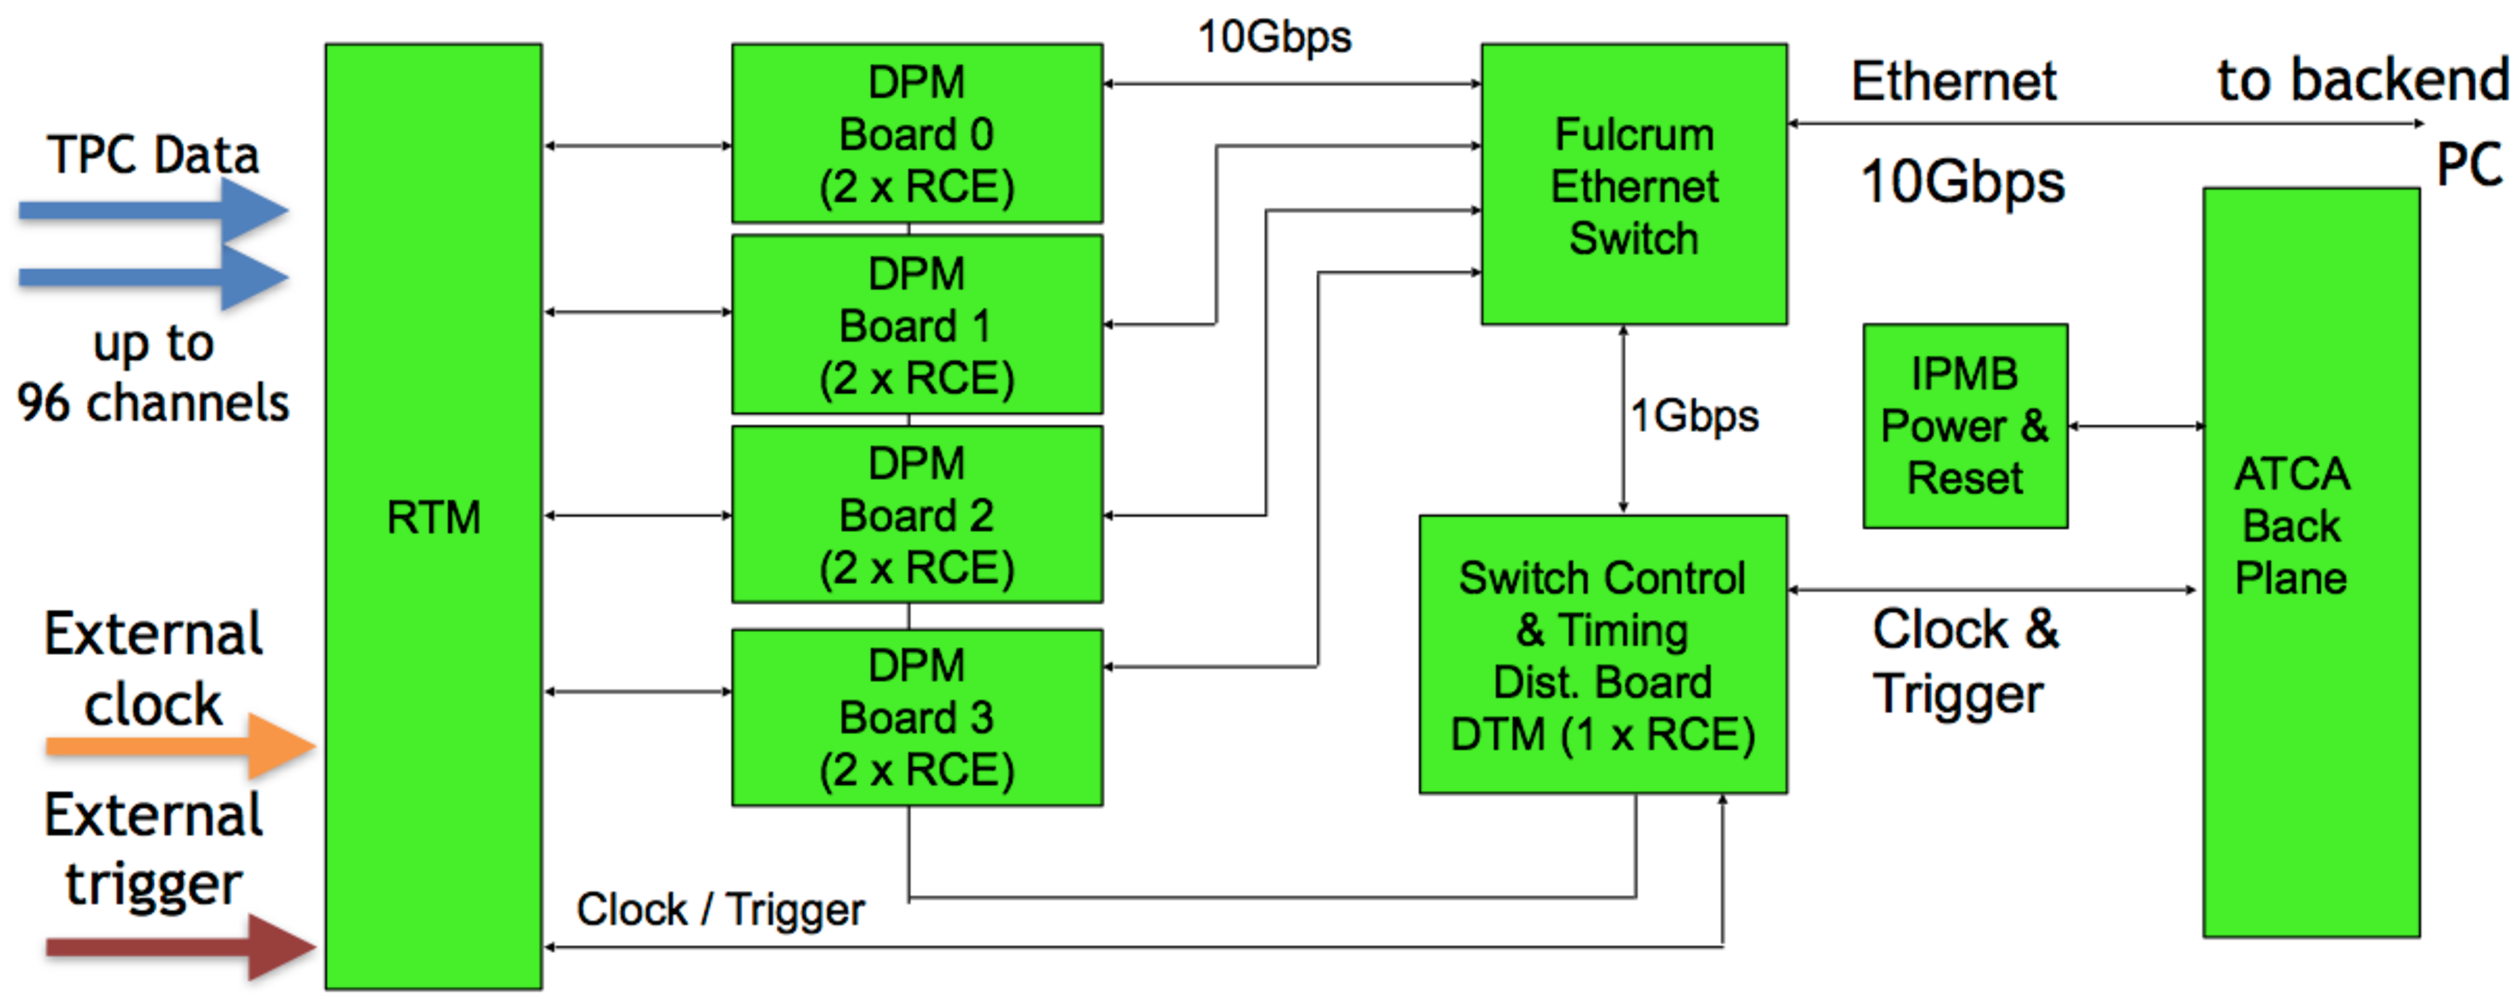
\includegraphics[scale=0.4]{figures/rce-block.pdf}
\label{fig:rceblock}
  \caption{Schematic for the TPC DAQ system.   }
\end{figure}


\begin{figure}[hbt]
  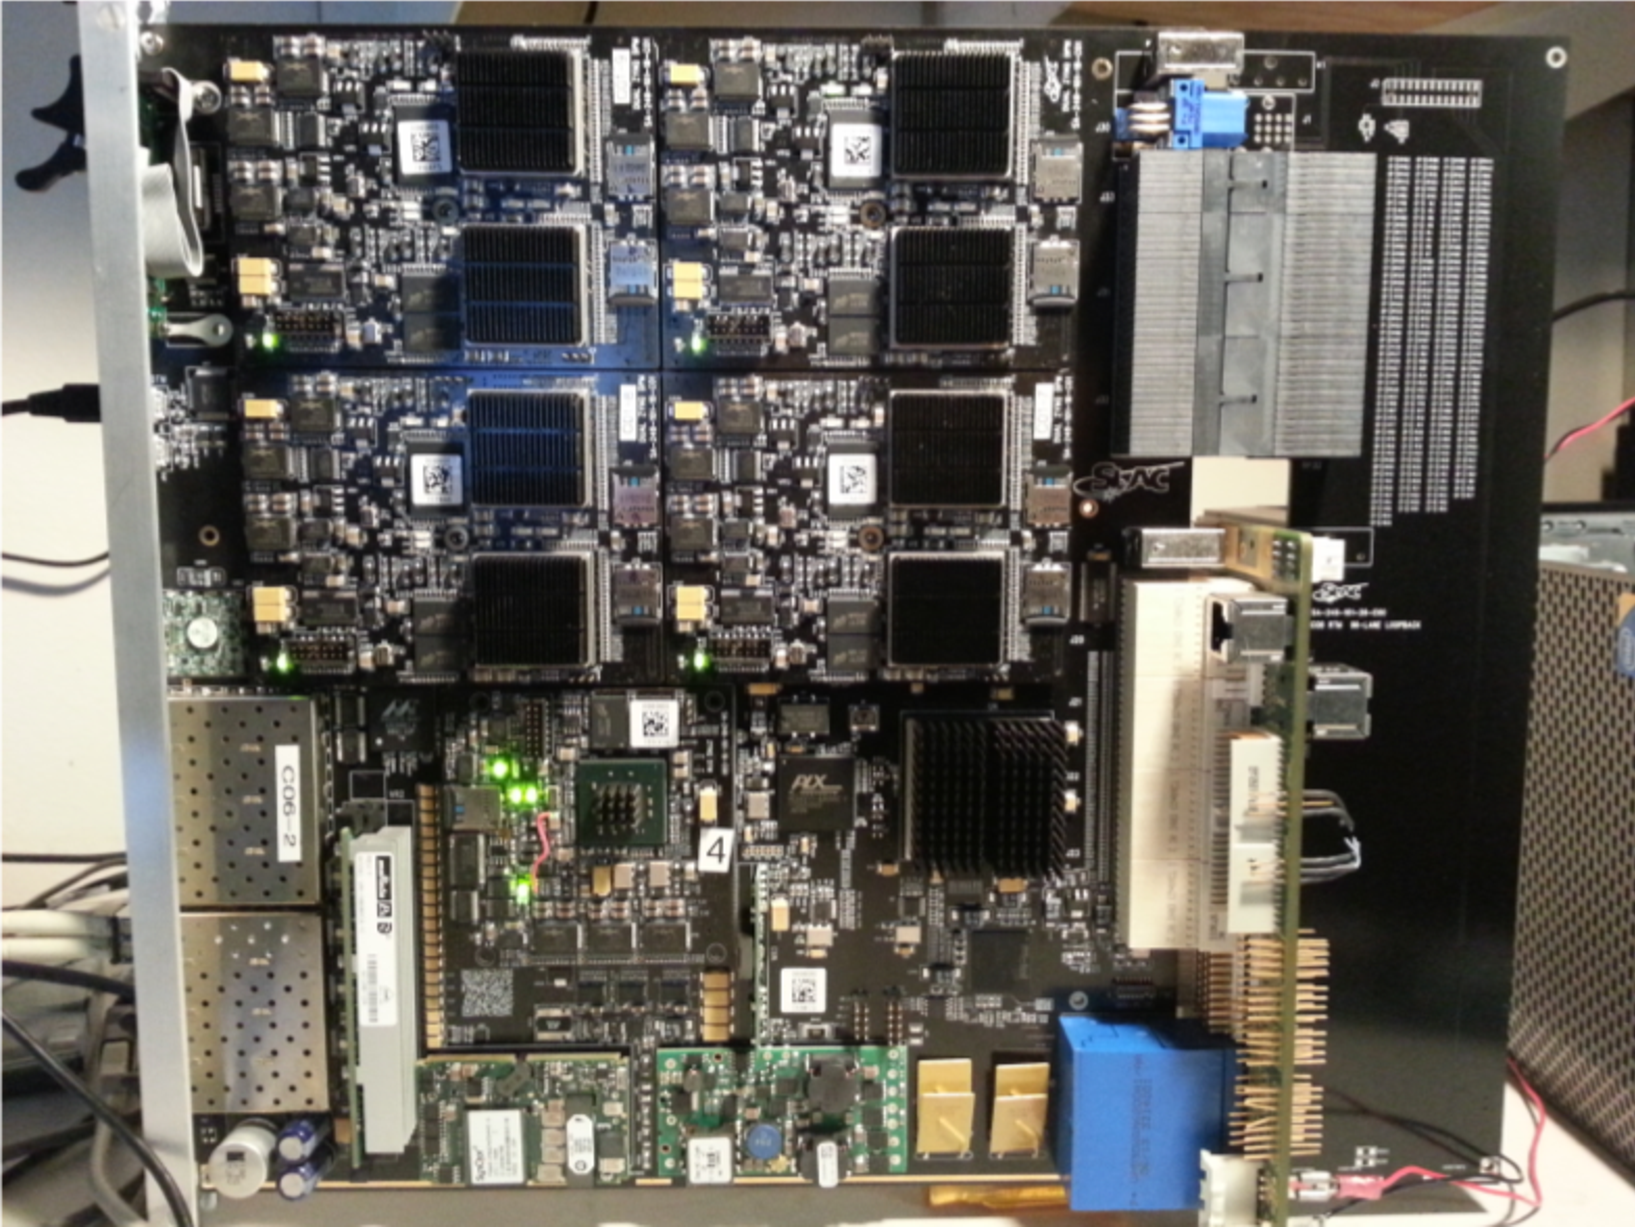
\includegraphics[scale=0.6]{figures/COB-gen3.pdf}
  \caption{\label{fig:cob} The COB (left of the large connectors) and RTM (right).  }
\end{figure}



